% The 1-skeleton of the torus: two loops e^1_a, e^1_b joined at e^0.
% Source: book/tex/homology/cellular.tex (§ Cellular homology of a torus).
\documentclass[border=2mm]{standalone}
\usepackage{tikz}
\usepackage{amssymb}
\usetikzlibrary{arrows.meta,decorations.markings}
\tikzset{midarrow/.style={postaction={decorate},decoration={
  markings,mark=at position 0.5 with {\arrow{Latex[length=2.4mm]}}}}}
\begin{document}
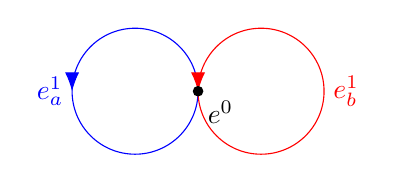
\begin{tikzpicture}[scale=0.8]
  \draw[blue, midarrow] (-1,0) circle (1);
  \draw[red, midarrow]  (1,0) circle (1);
  \node[blue] at (-2.35,0) {$e^1_a$};
  \node[red]  at (2.35,0)  {$e^1_b$};
  \fill (0,0) circle (2.4pt);
  \node[below right] at (0,0) {$e^0$};
\end{tikzpicture}
\end{document}
